\section{Point-source matching}
\label{sec:point-source-matching}

\subsection{Motivation}

For sectors with point-source emissions, the downscaling problem is not
limited to deciding how much mass belongs to an inventory point. A more
fundamental difficulty is that CAMS point coordinates do not always
localise the emitting facility precisely. They may fall near the
facility, in the centre of a coarse inventory cell, or at a location that
is spatially displaced from the real industrial installation. Directly
burning these coordinates into the high-resolution proxy grid would
therefore transfer the inventory mass to a location that is not
necessarily the physical source.

The point-source workflow was introduced to correct this limitation as
far as the available facility data allow. Each CAMS point is treated as
an inventory representation of an emitting source. It is then compared
with external facility records that describe real installations. The
objective is not to change the CAMS emission mass, but to identify the
most plausible real-world location to which that mass should be linked.
This distinction is important for later downscaling: the inventory point
preserves traceability to CAMS, while the matched facility provides the
spatial location used to represent the source more realistically.

\subsection{General matching procedure}

The matching workflow starts from the CAMS point-source records selected
for a given GNFR sector, country, year, and representative pollutant. The
representative pollutant is used to rank or filter the CAMS points when
a sector contains many possible records. Candidate facilities are then
assembled from the external dataset most appropriate for the sector. As
far as possible, the external facility sources are selected to remain
consistent with the point-source information reported for the CAMS-REG
inventory compilation \citep{CAMS-REG-v4}. The objective is to avoid
introducing a second, unrelated facility geography while still correcting
the local displacement of the CAMS point coordinates. The datasets are
described in Appendix~\ref{app:datasets}.

For each CAMS point, nearby candidate facilities are screened within a
maximum search distance. This threshold is a hard constraint: a facility
located farther away than the sector-specific maximum distance is not
considered a possible match, even if it has a compatible activity or
pollutant. Candidate pairs that pass this distance screen are then scored
using three criteria. The first criterion is geographical proximity:
shorter distances increase the likelihood that a facility is the correct
match. The second criterion is pollutant consistency: a facility
reporting the same or a closely related pollutant receives a higher score
than a facility with no relevant pollutant information. The third
criterion is activity consistency: facilities belonging to the expected
industrial or sectoral activity class are preferred over facilities from
unrelated activities.

In generic form, the score for a CAMS point--facility pair can be written
as

\begin{equation}
  q =
  \beta_d q_d +
  \beta_p q_p +
  \beta_a q_a ,
\end{equation}

where $q_d$ is the distance score, $q_p$ the pollutant-consistency score,
$q_a$ the activity-consistency score, and the coefficients $\beta_d$,
$\beta_p$, and $\beta_a$ define their relative importance. Distance is
the primary constraint because very distant links are physically
unlikely, while pollutant and activity terms help distinguish between
nearby facilities in industrial clusters.

The same strict and fallback scoring weights are used for all matched
sectors. The sector-specific parameter is the maximum allowed
matching distance, which reflects the expected spatial uncertainty and
facility density of each sector.

\begin{table}[htbp]
  \centering
  \caption{Scoring weights used in the point-source matching procedure.}
  \label{tab:point-source-scoring-weights}
  \begin{tabular}{lccccc}
    \toprule
    Matching stage & $\beta_d$ & $\beta_p$ & $\beta_a$ & Minimum score & Candidate count \\
    \midrule
    Strict & 0.50 & 0.30 & 0.20 & 0.40 & 25 \\
    Fallback & 0.75 & 0.15 & 0.10 & 0.25 & 60 \\
    \bottomrule
  \end{tabular}
\end{table}

The matching is performed in descending order of CAMS point magnitude so
that the largest inventory sources are assigned first. A facility can be
assigned to only one CAMS point, which avoids duplicating the same real
installation across several inventory records. If no sufficiently strong
strict match is found, a fallback stage allows a weaker but still
distance-limited match. This fallback is useful for sectors where the
external facility dataset is incomplete or where facility names and
activity classifications are not fully harmonised across reporting
systems.

\begin{figure}[htbp]
  \centering
  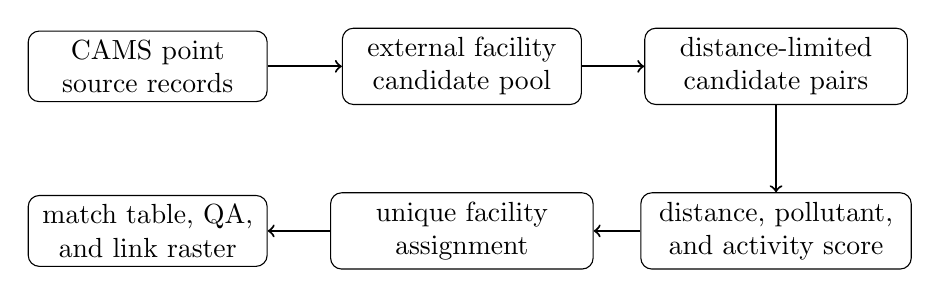
\begin{tikzpicture}[x=0.95cm,y=0.95cm]
    \node[draw, rounded corners, align=center, text width=2.8cm] (cams) at (0,0)
      {CAMS point\\source records};
    \node[draw, rounded corners, align=center, text width=2.8cm] (fac) at (4.2,0)
      {external facility\\candidate pool};
    \node[draw, rounded corners, align=center, text width=3.1cm] (screen) at (8.4,0)
      {distance-limited\\candidate pairs};
    \node[draw, rounded corners, align=center, text width=3.2cm] (score) at (8.4,-2.2)
      {distance, pollutant,\\and activity score};
    \node[draw, rounded corners, align=center, text width=3.1cm] (assign) at (4.2,-2.2)
      {unique facility\\assignment};
    \node[draw, rounded corners, align=center, text width=2.8cm] (out) at (0,-2.2)
      {match table, QA,\\and link raster};

    \draw[->, line width=0.75pt] (cams) -- (fac);
    \draw[->, line width=0.75pt] (fac) -- (screen);
    \draw[->, line width=0.75pt] (screen) -- (score);
    \draw[->, line width=0.75pt] (score) -- (assign);
    \draw[->, line width=0.75pt] (assign) -- (out);
  \end{tikzpicture}
  \caption{General point-source matching workflow. CAMS point records are compared with sector-specific facility candidates, screened by distance, scored using spatial and activity information, and written to diagnostic outputs.}
  \label{fig:point-source-matching-workflow}
\end{figure}

\subsection{Sector-specific facility datasets}

The facility dataset used for matching depends on the sector. This is a
methodological choice rather than a purely technical one: a good match
requires an external dataset whose facilities correspond to the physical
process represented by the CAMS point source. The choice follows the
facility sources reported for CAMS-REG point emissions where possible
\citep{CAMS-REG-v4}, and uses the dataset descriptions given in
Appendix~\ref{app:datasets} for traceability. The matching pollutant is
chosen from the CAMS point-source contribution of each sector, using the
pollutant that best represents the dominant or most diagnostic facility
signal.

\begin{table}[htbp]
  \centering
  \caption{External facility datasets used for point-source matching.}
  \label{tab:point-source-facility-datasets}
  \footnotesize
  \begin{tabular}{p{0.17\textwidth} p{0.27\textwidth} p{0.13\textwidth} p{0.13\textwidth} p{0.20\textwidth}}
    \toprule
    Sector & Facility dataset & Matching pollutant & Maximum distance & Rationale \\
    \midrule
    Public power & JRC Open Power Plants Database & CO & 20 km & CAMS power-point source basis \\
    Industry & E-PRTR and Industrial Emissions reporting & NO$_x$ & 25 km & CAMS industrial point-source basis \\
    Fugitive emissions & E-PRTR and Industrial Emissions reporting & CH$_4$ & 25 km & Energy, mineral, and chemical facilities \\
    Waste & E-PRTR and Urban Waste Water Treatment Directive reporting & CH$_4$ & 12 km & Waste facilities and treatment plants \\
    Solvents & E-PRTR and Industrial Emissions reporting & NMVOC & 10 km & Reported NMVOC-emitting facilities \\
    \bottomrule
  \end{tabular}
\end{table}

For public power, the facility pool is restricted to combustion-related
power plants, excluding non-combustion generation technologies when they
are not relevant for air-pollutant emissions. For industry, the matching
uses industrial reporting facilities and gives preference to activity
classes consistent with industrial combustion and process emissions. For
fugitive emissions, the matching also uses industrial reporting
facilities, but favours energy, mineral, and chemical activities because
these are the most relevant reported facility classes for point-like
fugitive sources. For waste, a combined facility pool is needed because
methane and other waste-sector emissions can originate from reported
waste installations and from waste-water treatment infrastructure. For
solvents, the sector is represented almost exclusively as an area source
in CAMS. However, the Greek CAMS inventory and the industrial reporting
data indicate that many facilities report NMVOC emissions, which
justifies retaining a point-source matching proxy for the facility-like
part of the solvent signal while treating the dominant residual component
through area-source subsector allocation.

\subsection{Two-location representation}

The matching output deliberately preserves both locations: the original
CAMS point and the matched real facility. This is the reason for
constructing a two-layer spatial product. The first layer burns the CAMS
point mass at the original inventory coordinate. The second layer burns
the same linked mass at the matched facility coordinate. Comparing the
two layers makes the spatial displacement visible and documents how much
mass is moved from the inventory point to the real-world installation.

This representation is useful for three reasons. First, it preserves
traceability to the CAMS point source, so the original inventory
information is not lost. Second, it provides the corrected facility-based
location used for high-resolution spatialisation. Third, it supports
quality control, because unusually long links, low scores, or systematic
offsets can be inspected visually before the matched point source is used
in the final downscaling workflow.


\begin{figure}[htbp]
  \centering
  \begin{subfigure}{0.48\textwidth}
    \centering
    \fbox{\begin{minipage}[c][4.0cm][c]{0.92\textwidth}
      \centering
      \includegraphics[width=0.7\textwidth]{figures/Proxies/Capture d'écran 2026-04-28 112834.png}
    \end{minipage}}
    \caption{Public power}
  \end{subfigure}
  \hfill
  \begin{subfigure}{0.48\textwidth}
    \centering
    \fbox{\begin{minipage}[c][4.0cm][c]{0.92\textwidth}
      \centering
      \includegraphics[width=0.7\textwidth]{figures/Proxies/Capture d'écran 2026-04-28 113004.png}
    \end{minipage}}
    \caption{Waste}
  \end{subfigure}
  \caption{Examples of CAMS point-source locations and matched facility locations. These maps are used to verify that the matched facility provides a more plausible physical location than the raw CAMS coordinate. In red the CAMS point location is shown, in blue the matched facility location is shown.}
  \label{fig:point-source-match-examples}
\end{figure}

\subsection{Quality-control outputs}

The point-source procedure produces tabular and spatial diagnostics. The
tabular match output records the CAMS point identifier, matched facility
identifier, coordinates of both locations, distance, score, matched
stage, selected pollutant value, and facility metadata where available.
The quality-control summary reports the number of CAMS points considered,
the number matched, the unmatched count, the coverage rate, and summary
statistics of match distance and score.

These diagnostics are part of the methodology because point-source
matching cannot be treated as a purely automatic operation. A high score
and short distance indicate that the external facility record is a
plausible spatial correction for the CAMS point. A low score or long
distance does not necessarily mean that the match is wrong, but it
signals that the result should be interpreted cautiously. The two-layer
spatial product and the example maps provide the visual counterpart to
the tabular QA, allowing the displacement between inventory coordinates
and facility coordinates to be inspected directly.
